\begin{abstract}

DNAproDB (\url{https://dnaprodb.usc.edu/}) is a widely used database, visualization tool, and processing pipeline for analyzing the structural features of protein–DNA interactions. Here we present a substantially updated version through additional data and functionalities. It contains an expanded volume of pre-analyzed protein–DNA structures, which will now be automatically updated weekly. The analysis pipeline now identifies water-mediated hydrogen bonds, and modified visualizations of protein–DNA incorporate this data. Tertiary structure-aware nucleotide layouts are now available. New file formats and external database annotations are supported. The website has been aesthetically modernized, and interactions with graphs and data is more intuitive. We also present a statistical analysis on the updated collection of structures revealing salient patterns in protein–DNA interactions. 

\end{abstract}

\section{Introduction}

Protein–DNA interactions play crucial roles in essential cellular functions like gene regulation, genome packaging, and DNA replication \citep{Spitz2012, Lai2017}. Diverse recognition mechanisms underlie these interactions \citep{rohs2009role, Rohs2010, Kitayner2010, Chiu2023}. Atomic resolution structures of protein–DNA complexes available in the Protein Data Bank (PDB) \citep{wwpdb2019protein} have been invaluable for understanding these readout mechanisms and provide insight that relate them to function. As a computational resource which extensively analyzes such structures and presents their data in publication-quality representations, the DNAproDB web server \citep{Sagendorf2017} and database \citep{Sagendorf2020} have been a useful resource for biologists, recognized by tool libraries such as the Nucleic Acid Knowledge Base (NAKB) \citep{Lawson2024}. 
This update improves the DNAproDB analysis pipeline, output data presentation, and web interface \hyperref[fig:dnaprodb1]{Fig. 4.1}. The updated analysis pipeline now computes annotations of water-mediated hydrogen bonds, which are known to play an important role \citep{Reddy2001} in protein–DNA recognition and, in some cases, a very prominent one \citep{Otwinowski1988}. Also, the pipeline now automatically processes and incorporates new PDB structures weekly. The primary interface visualization, ‘Residue contact map,’ now allows users to select a mapping algorithm for nucleic acid layout. In addition to secondary structure-based mapping \citep{Lorenz2011}, tertiary-structure aware mapping \citep{Mitra2024rnascape} is now available. Binding specificity data for transcription factors cataloged in the JASPAR2024 \citep{Rauluseviciute2024} database has been integrated. Users can now upload structures in the macromolecular Crystallographic Information File (mmCIF) format and download interface visualizations in an editable figure format. More information regarding these updates, as well as quality-of-life and user-interface improvements, is described in the following sections.
We analyzed the expanded DNAproDB structure collection for salient features of protein–DNA interactions (\hyperref[fig:dnaprodb2]{Fig. 4.2}). These results (based on a larger sample size in this update) reaffirm previous statistics presented about DNA minor groove recognition \citep{rohs2009role} and patterns of amino acid-base stacking for single stranded DNA presented \citep{Sagendorf2020}. Additionally, we present and discuss examples of the newly added water-mediated hydrogen bond annotations in selected structures (\hyperref[fig:dnaprodb3]{Fig. 4.3}).
DNAproDB has been used by experimental biologists to upload, analyze, and present interface visualizations in their work \citep{Webb2024}. We developed this update to assist their efforts, likely leading to additional contributions from the scientific community. We want to emphasize the increased utility of DNAproDB in light of structure prediction tools like AlphaFold3 \citep{Abramson2024}, RoseTTAFoldNA \citep{baek2024na}, and RoseTTAFold-AA \citep{Krishna2024}, and binding specificity prediction tools including DeepPBS \citep{Mitra2024} and rCLAMPS \citep{Wetzel2022}. These computational tools hint towards a promising future of protein–DNA structure prediction and design \citep{Glasscock2023}. We expect that DNAproDB will be an invaluable tool and assist such efforts. This work is led by me, with contributions from Ari S. Cohen, Dr. Jared M. Sagendorf, Prof. Helen Berman and supervised by Prof. Remo Rohs.

\begin{center}
    \begin{figure}
    \makebox[\textwidth]{\includegraphics[width=0.8\paperwidth]{./dnaprodbfigs/figure1.png}}
 % archetecture.png: 1149x508 px, 72dpi, 40.53x17.92 cm, bb=0 0 1149 508
        \caption[Key aspects of this update to DNAproDB.]{\textbf{Key aspects of this update to DNAproDB.} ({\bf A}) Automatic update and separated external annotation incorporation scheme.  ({\bf B})  Different nucleic acid layout options, with added tertiary structure aware RNAscape layout, shown for PDB ID: 3LDY. ({\bf C}) Water-mediated hydrogen bond annotation. ({\bf D}) Various improvements in other aspects of DNAproDB. }
  \label{fig:dnaprodb1}
\end{figure}
\end{center}


\section{Update details}

\subsection{Processing pipeline and data update}
At the time of its previous release \citep{Sagendorf2020}, DNAproDB contained a static collection of structures. This resulted in newly released structures being unavailable. In this update, we have addressed this limitation by implementing an automatic update pipeline (\hyperref[fig:dnaprodb1]{Fig. 4.1A}). Every weekend, the pipeline queries the PDB for newly released structures, downloads and processes them, and adds them to the DNAproDB collection. 
In addition, the structure processing pipeline has been separated from any external annotation dependency. This allows external annotations to be updated without reprocessing each structure or affecting the user experience. Annotations from the JASPAR2024 \citep{Rauluseviciute2024} database (incorporating the most recent binding specificity matrix ID and logo) have been included whenever applicable. 
The asymmetric unit molecular weight cutoff, which determines whether a structure is included in the collection, has been expanded from 250 to 1500 kDa, increasing the structures available for analysis. The latest collection size as of June 7th, 2024, is 6,731 structures. This set has been analyzed and was included in the results presented in \hyperref[fig:dnaprodb2]{Fig. 4.2}. 
Originally, a large part of the processing pipeline was written using Python 2 \citep{Guido1995}. However, support for Python 2 is no longer available by the open-source community as of January 1, 2020, and Python 3 \citep{Guido2009} has become the new standard. We redesigned the backend processing pipeline to ensure compatibility with Python 3. 
As an expansion of available features, water-mediated hydrogen bonds between protein and DNA have been calculated and annotated within this update. The program HBPLUS \citep{McDonald1994}, with the ‘-h’ option set to 3 \AA, and the ‘-d’ option set to 3.5 \AA, and with the remaining parameters set as default, is used to detect hydrogen bonds. Custom scripts were written to determine water-mediated interactions via shared water molecules between hydrogen-bonded pairs (see Data Availability).  

\subsection{Visualization}
We updated the ‘Residue contact map’ and ‘3D structure’ (\hyperref[fig:dnaprodb1]{Fig. 4.1B}) visualizations presented in DNAproDB in several ways. The nucleic acid backbone color used in these components has been changed to a more visually pleasing metallic blue-gray color, compared to the previously used yellow-orange color. 
In addition to the previous secondary-structure-based and circular layouts, an RNAscape \citep{Mitra2024rnascape} based layout for placing nucleic acids has been computed and added to the ‘Residue contact map’. This new layout is more representative of tertiary structure compared to the other two representations (\hyperref[fig:dnaprodb1]{Fig. 4.1B}). An option to switch between these different layouts is available.
During this update, some Python 2 version utilities for secondary structure-based layout computation were discontinued. We replaced these utilities with analogous Python 3 versions provided by the ‘Forgi’ \citep{Thiel2019} package. 
Water-mediated hydrogen bonds have now been incorporated as an interaction edge in the ‘Residue contact map’. These are indicated by a black circle (\hyperref[fig:dnaprodb1]{Fig. 4.1C}) in the interaction map. Hovering over the water-mediated contacts will present further information (e.g., residue number of the water molecule involved). An option to hide these interactions is also available. The ‘3D structure’ component now displays the solvent alongside the structure (in a previous version, the solvent was removed). A button to hide solvent is included. 

\subsection{Web interface and user experience}

Since its inception, we have continuously provided support for DNAproDB users and taken note of their feedback. In this update, we redesigned the web interface based on this information (\hyperref[fig:dnaprodb1]{Fig. 4.1D}). Textual clutter has been reduced on the home page and report pages for each structure. Instructions and explanations for different components, which were previously written directly on the page, are now available as pop-up components upon mouse hover. Report pages for each PDB entry now prominently display the title of the entry. The information tables have been rearranged in a modern and tabular fashion, resulting in further decluttering of information. 
DNAproDB offers many customization features for the Residue contact map. However, these options were often overlooked by users due to their non-prominent placement on the website. We have redesigned the user interface to make basic options like rotation, zooming, download, and switching between the layout algorithms easily accessible directly above the visualization. Buttons to access further customization options (‘Chart options’ and ‘Interface selection’) are prominently placed. The options within the ‘Chart options’ tab have been expanded. Within the ‘Interface selection’ tab, basic options (model, entity, chain, moiety selection) are shown first. Additional options are presented as advanced options. Mouse-based interaction controls for the ‘3D viewer’ and ‘Residue contact map’ have been made analogous, as much as possible.
The download option now supports the editable Scalable Vector Graphics (SVG) format. DNAproDB currently displays Watson-Crick, Hoogsteen, and other base-pairing geometries via correspondingly stylized base-pairing edges (e.g., Hoogsteen base-pairing in p53-tetramer-DNA complex \citep{Kitayner2010} reflected in \hyperref[fig:dnaprodb3]{Fig. 4.3E}). For additional analysis of non-Watson-Crick base-pairing geometries, a link to the RNAscape \citep{Mitra2024rnascape} webserver has been included in each report page. Clicking this link will redirect the user to the RNAscape website and automatically run it on the desired structure.

\subsection{Quantitative analysis of readout features}
Entries in the DNAproDB collection (as of June 7th, 2024) encompass protein–DNA structures including single-stranded (ssDNA), double-stranded DNA (dsDNA), and other conformations (e.g., G-quadruplex). We quantified the growth of such entries over time based on their PDB release dates, which reflects an exponential trend (\hyperref[fig:dnaprodb2]{Fig. 4.2A}). Fewer entries contain ssDNA and other conformations compared to dsDNA. However, recent years (2016 onwards) demonstrate a steady growth also in ssDNA entries (\hyperref[fig:dnaprodb2]{Fig. 4.2A}). 
Studies on protein-DNA structures have revealed consistent patterns in protein residue–DNA interaction frequencies \citep{rohs2009role, Lin2019}. We sought to quantify similar statistics in the updated collection of DNAproDB. To this end, we computed relative abundances of different amino acids interacting with the major groove (\hyperref[fig:dnaprodb2]{Fig. 4.2B}), minor groove (\hyperref[fig:dnaprodb2]{Fig. 4.2C}), and phosphodiester backbone (\hyperref[fig:dnaprodb2]{Fig. 4.2D}). Relative abundance for a residue (R) is the fraction of appearance of this protein residue in an interaction with a DNA moiety relative to other residues. 
\begin{align}
\text{Relative abundance (R)} = \frac{|\text{interactions involving R}|}{\sum\limits_\text{R}|\text{interactions involving R}|}
\end{align}
\begin{center}
    \begin{figure}
    \makebox[\textwidth]{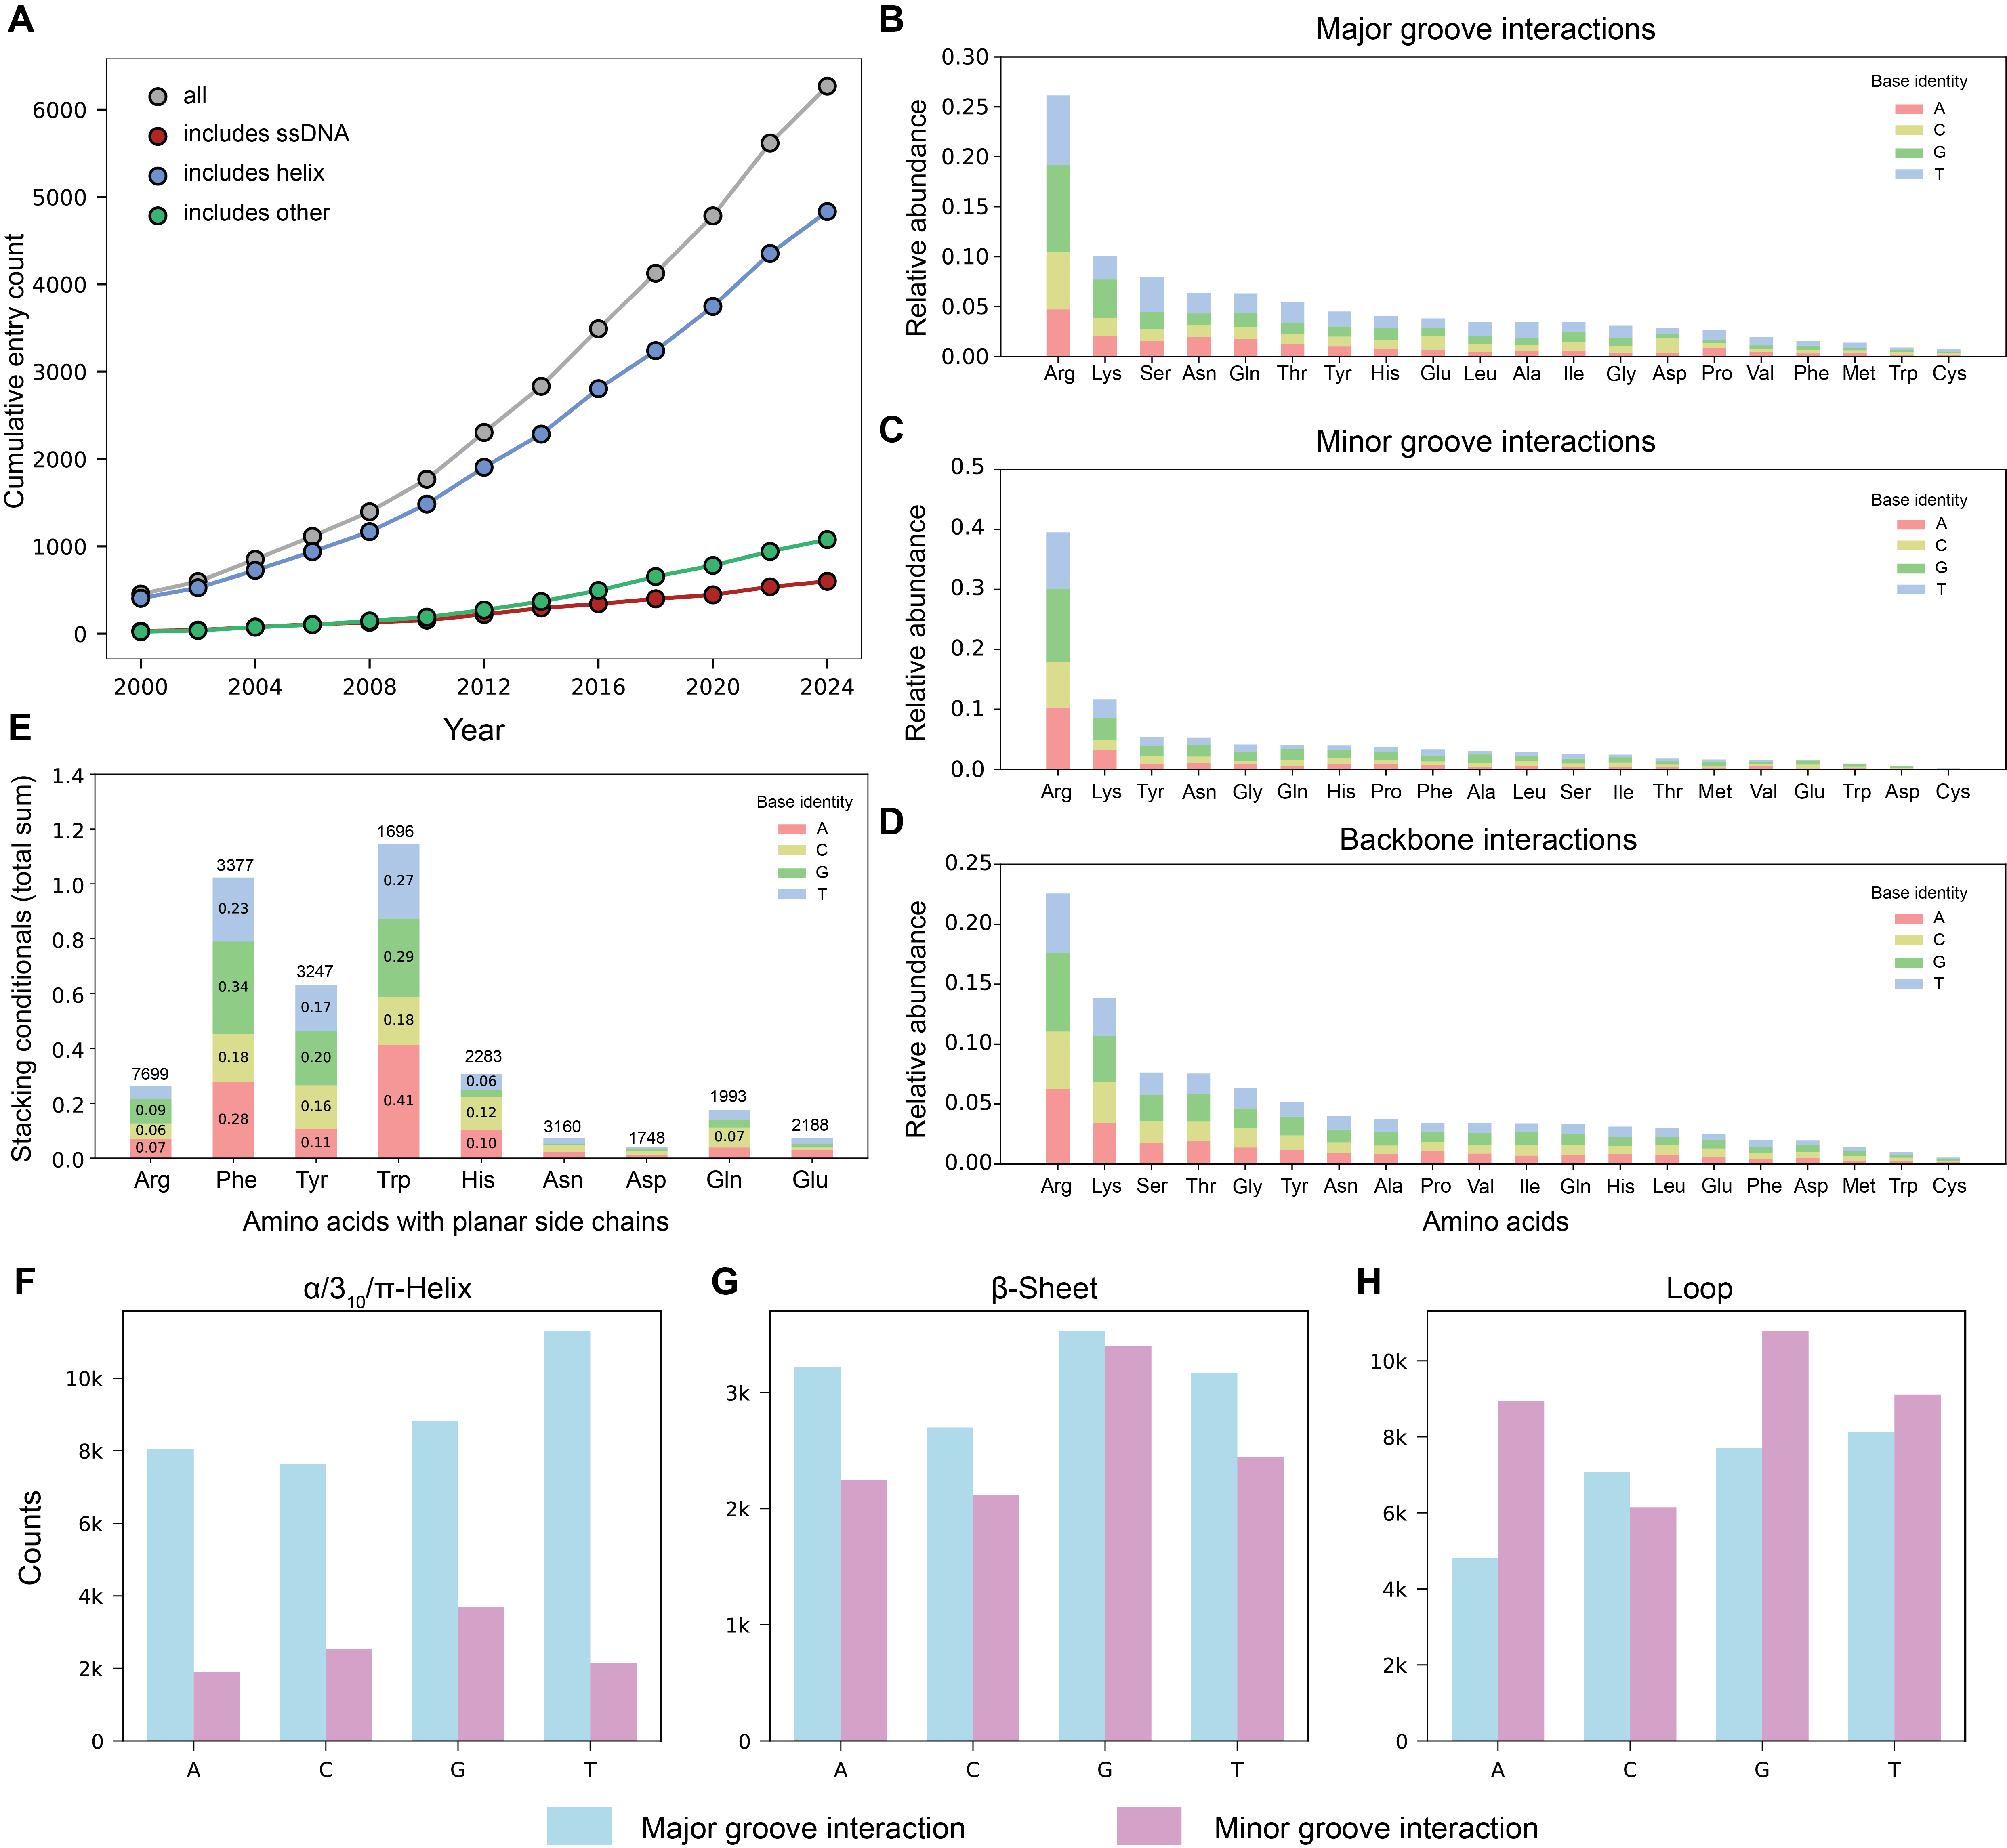
\includegraphics[width=0.8\paperwidth]{./dnaprodbfigs/figure2.png}}
 % archetecture.png: 1149x508 px, 72dpi, 40.53x17.92 cm, bb=0 0 1149 508
        \caption[Quantitative analysis of protein–DNA complexes in the DNAproDB collection. ]{\textbf{Quantitative analysis of protein–DNA complexes in the DNAproDB collection. } ({\bf A}) PDB release years of structures catalogued in the updated DNAproDB collection (as of June 7th, 2024). ({\bf B-D})   Relative abundance of different amino acids interacting with DNA major groove (B), minor groove (C), and phosphodiester backbone (D). ({\bf E}) Conditional probabilities of different protein residues and base forming a stacking geometry. Y-axis represents summed values over the bases for each amino acid.({\bf F-H}) Counts of interactions with different bases, categorized by major and minor groove for secondary structure classes: Helix (includes $\alpha$/$3_{10}$/$\pi$-helix) (F), Sheet ($\beta$-sheet) (G) and loop residues (H) }
  \label{fig:dnaprodb2}
\end{figure}
\end{center}
This is computed separately for the major groove, minor groove, and DNA backbone. Each of these values in \hyperref[fig:dnaprodb2]{Fig. 4.2B-E} is further subdivided into fractions per DNA base, shown in four colors. For the major groove, we see an abundance of residues able to perform recognition via hydrogen bonds with arginine (Arg) and lysine (Lys) residues showing the greatest presence (\hyperref[fig:dnaprodb2]{Fig. 4.2B}). For the minor groove, this preference for arginine and lysine is even stronger relative to other residues (\hyperref[fig:dnaprodb2]{Fig. 4.2C}). This agrees with the observation that the minor groove is more electronegative \citep{rohs2009role}, favoring positively charged amino acid sidechains while repelling negatively charged sidechains (e.g., aspartic acid (Asp), glutamic acid (Glu) etc.). 
For amino acid residues (R) with a planar side chain component (i.e., able to form a stacking interaction with a base (B $\in$ [A,C,G,T]) in single-stranded DNA), interaction geometries (g) can be of three types: g $\in$ [stack, pseudo pair, other]. Stacking conditionals P(g=stack $|$ R, B) were computed for major and minor groove interactions as a fraction of the counts of stack geometry against counts for all geometries. i.e.,
\begin{align}
P(\text{g=stack} | \text{R, B})= \frac{|\text{g=stack, R,B}|}{\sum\limits_\text{g}|\text{g, R, B}| }
\end{align}
This information is presented in \hyperref[fig:dnaprodb2]{Fig. 4.2E} in the form of a stacked bar chart. The total height of each stacked bar (i.e., for each amino acid) is $\sum\limits_\text{B}P(\text{g=stack} | \text{R, B})$ . The pattern visible in this data conforms with the previously computed version in \citep{Sagendorf2020} while encompassing a larger sample size.
DNAproDB also provides annotations and a visualization (‘Helical contact map’) reflecting how various secondary structure elements of a protein interact with the major and minor groove of DNA. We quantified these interactions to reveal statistical patterns (\hyperref[fig:dnaprodb2]{Fig. 4.2F-H}). We compute instances of helical secondary structures (including $\alpha$-helices, $3_{10}$-helices, and $\pi$-helices) interacting with the four primary DNA bases in either the major or minor groove (\hyperref[fig:dnaprodb2]{Fig. 4.2F}). There is a clear preference for the major groove for protein helices, reflecting the use of a recognition helix by many protein families \citep{Garvie2001}. On the other hand, for $\beta$-sheets, major and minor groove interactions are comparable in number, with a slight preference for the major groove (\hyperref[fig:dnaprodb2]{Fig. 4.2G}). The ‘loop’ category reflects residues appearing in loop regions of proteins interacting with DNA. Minor groove interactions are slightly more favored in this case (\hyperref[fig:dnaprodb2]{Fig. 4.2H}). In all cases, guanine (G) is the most favored DNA base that is contacted. 

\subsection{Water-mediated hydrogen bonds}
As described previously, the updated DNAproDB processing pipeline detects and visually annotates (\hyperref[fig:dnaprodb1]{Fig. 4.1B}) water-mediated hydrogen bond interactions between protein and DNA. This feature improves the accuracy and relevance of the DNAproDB visualization for some structures. For example, the co-crystal structure of the Trp repressor/operator complex (PDB ID: 1TRO, \hyperref[fig:dnaprodb3]{Fig. 4.3A}, Residue contact map: \hyperref[fig:dnaprodb3]{Fig. 4.3B}) reflects a protein–DNA recognition scheme without any direct hydrogen bonds in the major and minor groove. Instead, DNA recognition occurs via water-mediated hydrogen bonds (\hyperref[fig:dnaprodb3]{Fig. 4.3B}) \citep{Otwinowski1988}. A detailed view of two protein backbone nitrogen atoms (belonging to Ile79 and Ala80) recognizing G11 in this manner is presented in \hyperref[fig:dnaprodb3]{Fig. 4.3C}. This type of recognition scheme was previously not reflected in DNAproDB. Similarly, protein residues interacting with DNA only through water-mediated hydrogen bonds were also not displayed in the Residue contact map. One such example is the p53 tetramer structure (PDB ID: 3KZ8 \citep{Kitayner2010}, \hyperref[fig:dnaprodb3]{Fig. 4.3D}, Residue contact map: \hyperref[fig:dnaprodb3]{Fig. 4.3E}). This structure illustrates serine residues (Ser121) near the tetramerization interfaces involved in water-mediated hydrogen bonds with the major groove edge of two G bases (shown for one selected base in \hyperref[fig:dnaprodb3]{Fig. 4.3F}). As this is the sole mode of interaction for these two residues, they were omitted from the visualization in the previous DNAproDB version \citep{Sagendorf2020}. In this update, these interactions are correctly shown. A variety of complex interaction geometries are possible when water-mediated hydrogen bonds are involved. One such example can be found in interactions of the RXR/RAR DNA-binding domain heterodimer in complex with the retinoic acid response element (PDB ID: 1DSZ \citep{Rastinejad2000}, \hyperref[fig:dnaprodb3]{Fig. 4.3G}, Residue contact map: \hyperref[fig:dnaprodb3]{Fig. 4.3H}). The lysine residue (Lys1260) is involved in recognizing consecutive bases (G and T) through water-mediated hydrogen bonds involving two different water molecules. This update to DNAproDB allows exploring such recognition schemes. 

\begin{center}
    \begin{figure}
    \makebox[\textwidth]{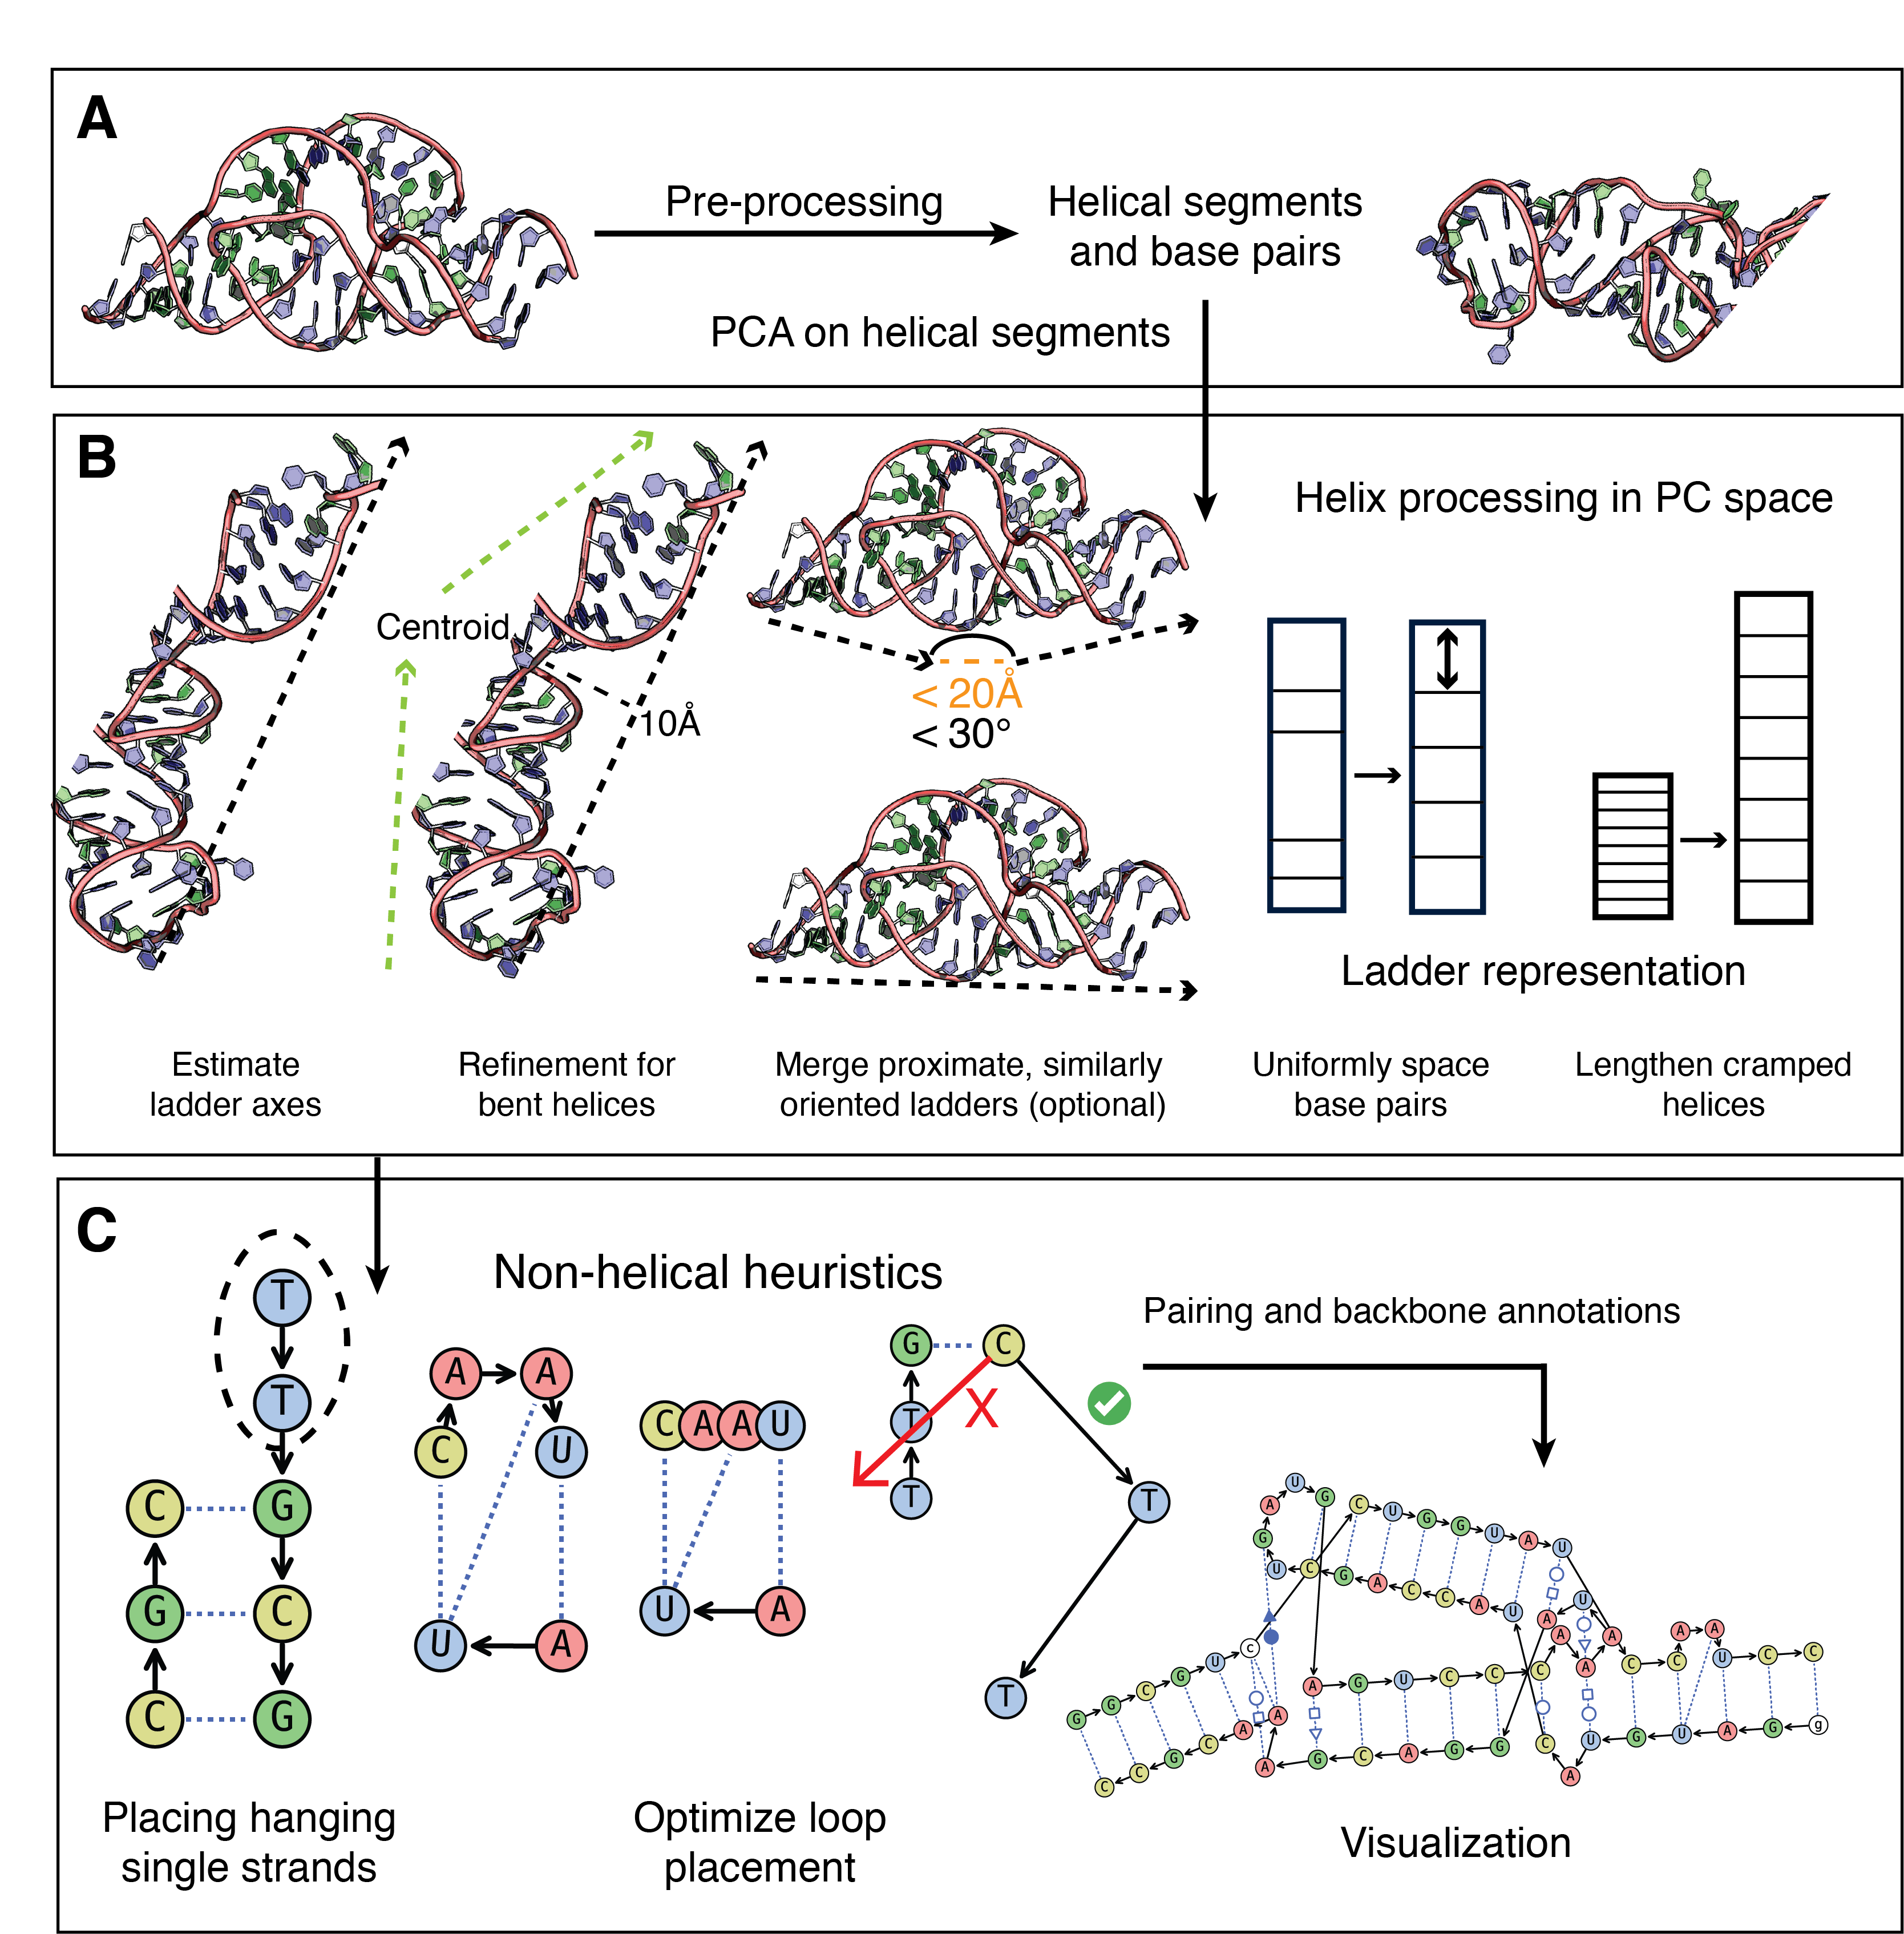
\includegraphics[width=0.8\paperwidth]{./dnaprodbfigs/figure3.png}}
 % archetecture.png: 1149x508 px, 72dpi, 40.53x17.92 cm, bb=0 0 1149 508
        \caption[Water-mediated hydrogen bond annotation in DNAproDB]{\textbf{Selected examples of water-mediated hydrogen bond annotations as reflected in the updated DNAproDB.  } ({\bf A-C}) Trp repressor/operator complex (PDB ID: 1TRO)  ({\bf D-F})    p53 tetramer with Hoogsteen base pairs (PDB ID: 3KZ8). ({\bf G-I}) Conditional probabilities of different protein residues and base forming a stacking geometry. Y-axis represents summed values over the bases for each amino acid.({\bf F-H}) RXR-RAR DNA-binding complex (PDB ID: 1DSZ). In each of the three cases, the 3D structure of the respective complex is shown in (A, D, G). The DNAproDB Residue contact map is shown (with only selected protein residues annotated) in (B, E, H). Atomic views of selected water-mediated hydrogen bond interactions are shown in (C, F, I), respectively. }
  \label{fig:dnaprodb3}
\end{figure}
\end{center}


\section{Discussion}
DNAproDB, since its inception in 2017 \citep{Sagendorf2017}, has been a valuable resource for the structural biology community. Its unique and extensive analysis pipeline, covering diverse aspects of protein–DNA binding, outputs data that can be readily used in downstream analysis by the user \citep{Sagendorf2020}. The interactive and publication-quality visualizations presented by DNAproDB have been used extensively by the structural biology community. In this update, we improved DNAproDB in multiple aspects. New structures released since the last update in 2019 \citep{Sagendorf2020} have been incorporated, resulting in a much larger collection. The pipeline has been future-proofed via the new automatic update feature. The backend implementation has been upgraded to Python 3, ensuring a long-lasting lifespan for DNAproDB. 
A key scientific improvement in the analysis pipeline is the incorporation of water-mediated hydrogen bond calculation. Interest in water-mediated interactions has been growing. This is evidenced by the CASP16 challenge for predicting solvent shells around the Tetrahymena ribozyme structure \citep{kryshtafovych2023critical}. Currently, these interactions are not well modeled by structure prediction and analysis tools \citep{Abramson2024, baek2024na, Krishna2024, Mitra2024, Jumper2021, Sagendorf2024}. We expect that this added feature in DNAproDB advances the field in the understanding of readout mechanisms. 
Visualizations have been improved by enabling tertiary structure-aware nucleic acid layouts, incorporation of water-mediated hydrogen bond indicators, greater customizability, and other aesthetic changes. The website style has been redesigned, and data presentation has been improved. Structure files in mmCIF format can now be uploaded, which was previously unsupported. Altogether, these updates result in an updated DNAproDB, which we expect to continue serving the structural biology community for the foreseeable future.

\subsection{Data availability}
DNAproDB is freely available for all users at \url{https://dnaprosb.usc.edu/}. The previous version remains available at \url{https://dnaprosb.usc.edu/v1/}. 
The pipeline and frontend implementations are available via GitHub:
\url{https://github.com/timkartar/DNAproDB}; 
\url{https://github.com/ariscohen/DNAproDB_frontend}
